% This file was created with tikzplotlib v0.10.1.
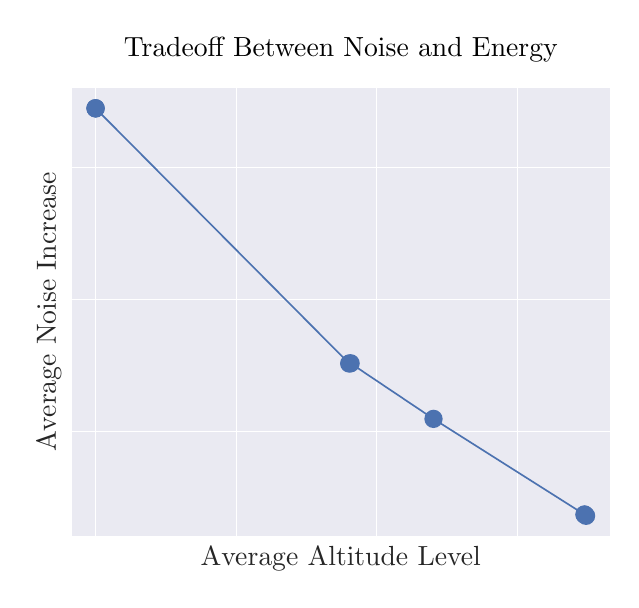
\begin{tikzpicture}

\definecolor{darkslategray38}{RGB}{38,38,38}
\definecolor{lavender234234242}{RGB}{234,234,242}
\definecolor{steelblue76114176}{RGB}{76,114,176}

\begin{axis}[
axis background/.style={fill=lavender234234242},
axis line style={white},
tick align=outside,
title={Tradeoff Between Noise and Energy},
x grid style={white},
xlabel=\textcolor{darkslategray38}{Average Altitude Level},
xmajorgrids,
xmajorticks=false,
xmin=912.832524232482, xmax=2830.82602762633,
xtick style={color=darkslategray38},
y grid style={white},
ylabel=\textcolor{darkslategray38}{Average Noise Increase},
ymajorgrids,
ymajorticks=false,
ymin=20.4190729579603, ymax=27.2081842470298,
ytick style={color=darkslategray38}
]
\addplot [semithick, steelblue76114176, mark=*, mark size=3, mark options={solid}]
table {%
1000.01404711402 26.8995882793448
1000.0278434845 26.8995123090261
1000.72596537843 26.8959457867238
1901.59520422678 23.0338842837022
1906.83530423816 23.0374524528488
2201.36718550651 22.1955750501913
2738.1970805585 20.746784072
2743.6445047448 20.7276689256453
2738.05149753261 20.7472194366616
};
\end{axis}

\end{tikzpicture}
